\documentclass[11pt]{report}

% imports
\usepackage{pdfpages}
\usepackage{graphicx}
\graphicspath{ {images/} }

\begin{document}

% init
\includepdf[pages=-,fitpaper=true]{EN_Forside_for_masteroppgave.pdf}
\pagenumbering{roman}

\chapter*{Abstract}
\addcontentsline{toc}{chapter}{Abstract}
Influenza epidemics costs both lives and a tremendeous amount of money for any country. Citizens that become sick are less productive and the overall quality of life is drastically reduced for the amount of the individuals period of illness as well as the community during a flu season. The ability to reduce the spread of infectious diseases saves both lives and resources. \\

This project aims to explore the possibilities to detect influenza outbreaks as soon as they are happening with the use of relevant datasets available. Information about different aspects of a citizens life on a grand scale reveals patterns and trends that could be linked to an epidemic outbreak, and thus prove useful for active measurements against further spread on a early debut. \\

The results show ...\\

Possible solutions to ...

\chapter*{Preface}
\addcontentsline{toc}{chapter}{Preface}
This thesis was written for the Department of Electrical Engineering and Computer Science at the University of Stavanger. Creating a means to solve  problems that limit peoples lives have always been a real motivator. Predicting the flu season and hindering it in early stages would save an enormous amount of resources and improve life quality, this would be very rewarding. A special thanks to the supervisor for this project from the University of Stavanger Erlend Tøssebro for his enthusiastic guidance and involvement, and the initiator who inspired incentive to the creation of this project as well as his continuous helpful guidance and involvement Phd fellow Lars Ole Grottenberg. 

\tableofcontents{}
\pagenumbering{arabic}
% ------------------------------------------------------------------------------------------------
\chapter*{\vspace{-3cm}1 Project Introduction}

\section*{1.1 Motivation}

\section*{1.2 Task}

\section*{1.3 Outline}

% ------------------------------------------------------------------------------------------------
\chapter*{\vspace{-3cm}2 Related Works}

\section*{2.1 TODO}

% ------------------------------------------------------------------------------------------------
\chapter*{\vspace{-3cm}3 Experimental}
In this chapter the different datasets used will be introduced. The goal of this project is to use as many datasets possible and then later evaluate them according to relevant results.

\section*{3.1 Folkehelseinstituttet}
The Institute of Public Health or Folkehelseinstituttet (fhi) have weekly updates\cite{fhi.no} on the development of the seasonal cases of influenza. The reports include numbers of diagnoses and graphs of flue-like illnesses. No numbers are appended to the flue-like illnesses and therefore this project will not take that into account, only diagnosed instances of influenza. Exact numbers are only included in the three last years, therefore the project only uses the seasons of the years 2015/2016, 2016/2017 and 2017/2018. The reports covers how many Norwegians seek treatment for influenza like illnesses and what kind of influenza viruses are circulating in the country, vaccine status and recommendations, as well as the overall prognosis of this season. The surveillance of influenza is based on doctors reporting flue-like illnesses of patients and testing those hospitalized for influenza viruses. Doctors report flue-like illnesses based on these symptoms: muscle pain, coughing, fever and the feeling of being sick.

\section*{3.2 Vegvesenet}
The Norwegian Public Roads Administration (NPRA), or Vegvesenet as it is called in Norwegian, have several different collections of data available for a number of different purposes. The motivation of this project requires traffic data of how many cars pass a certain registration station at a given time at a given position, the hypothesis for this that when people are ill they commute less and thus this shows on statistical data. Freely on their website \cite{vegvesen_for_utviklere} there are a few interesting options for this project. They have traffic information in a DATEX API, statistics in XLM and traffic index data relevant to the years before. It is important that the data collected is on a weekly basis atleast in order to compare it to the influenza data. The data on their website does not suffice for this purpose, traffic data is only registered on a yearly and monthly basis. Luckily upon further investigation and help from the NPRA better data was granted upon request, hidden from that available on their website. The data given contained a set of traffic registration stations throughout Norway. With this statistics of the daily traffic amount and spatial bounds can be derived showing the possible correlation influenza can have on traffic.

\section*{3.3 Twitter}
The reason twitter data is interesting is that it contains self reported instances of influenza before the patient or even if the patient visits a doctor for diagnosis and treatment. The pros are instant notification about possible influenza like illness and its spread against the cons of it being self reported. Twitter have several APIs available for public use, the one used in this project is the REST or search API which allows for searching against a set of keywords. The REST API is limited though, data accessible is only max 10 days old and the search limit is on a max of one hundred messages called 'tweets'. The other API of interest is the stream API which continually gets the latest tweets. In order to only get Norwegian tweets a set of geographical locations needs to be defined. The reason the stream API was not used is firstly because it requires a computer running on the internet continuously in order to get all the tweets. Secondly the data collected could become large slowing down other post-processing algorithms and taking up unnecessary storage. Lastly the stream API only provides a small set of the actual tweets tweeted, this means when searching for a specific term using the stream API some relevant tweets could go unnoticed and thus a search API is more appropriate for this task.

% ------------------------------------------------------------------------------------------------
\chapter*{\vspace{-3cm}4 Implementation}

\section*{4.1 Folkehelseinstituttet}
From the datasets available it was a simple job to plot the data in a graph. Figure \ref{fig:infstat} show the three last seasons of influenza. The plotting was done manually as fhi only provides the data in pdf format.

\begin{figure}[ht]
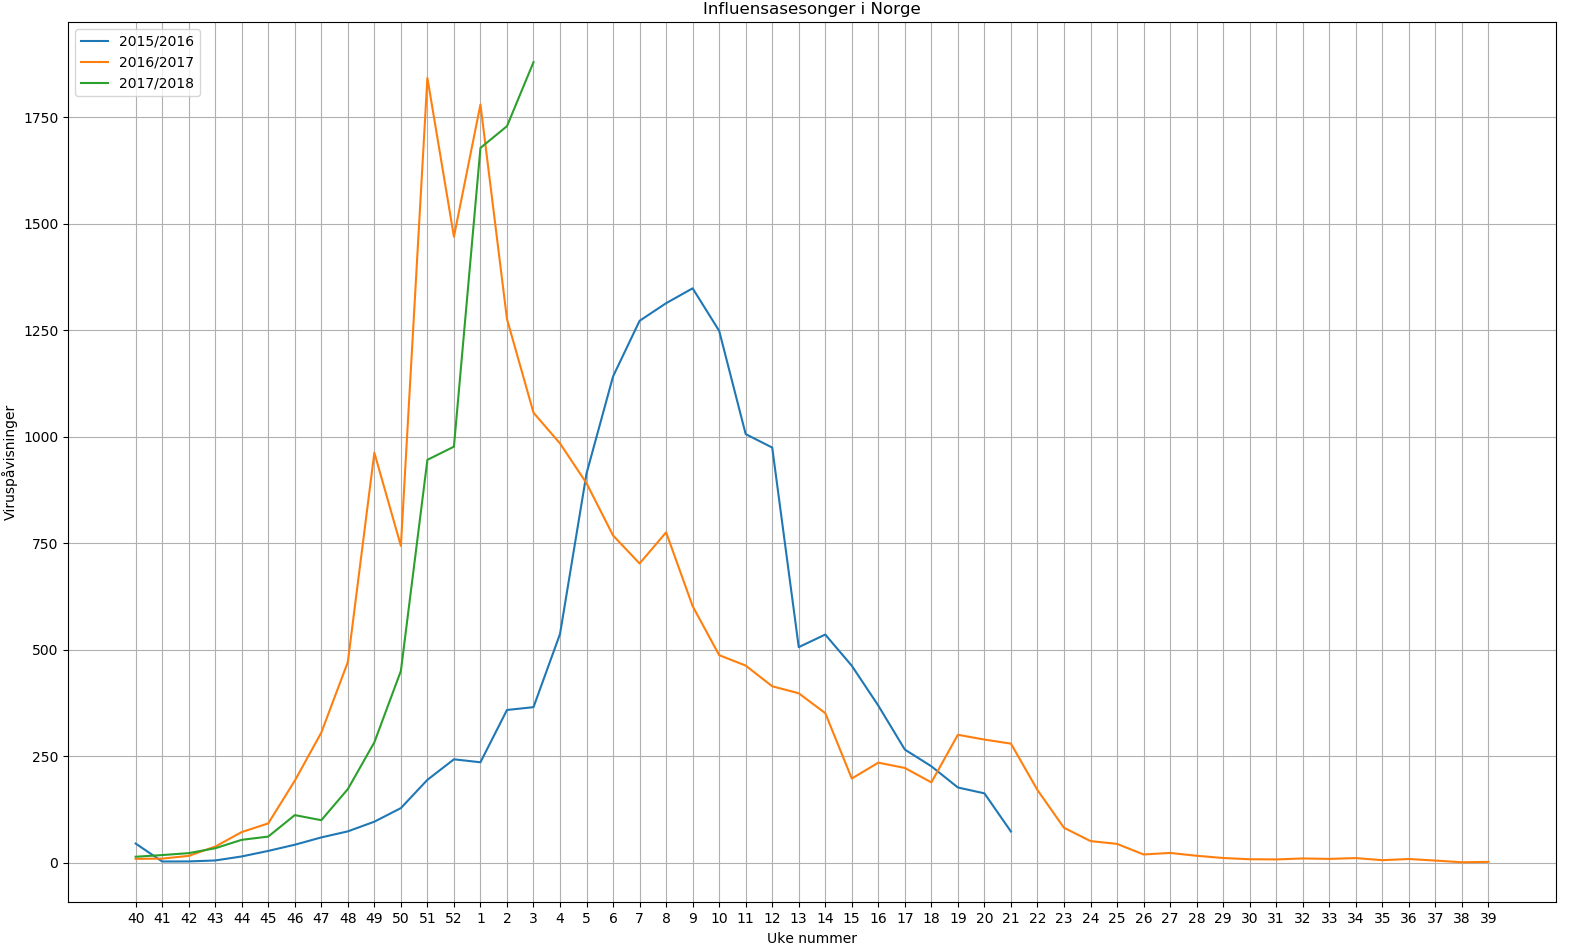
\includegraphics[width=16cm]{influenza_15_till_18}
\centering
\caption{Influenza seasons}
\label{fig:infstat}
\end{figure}

\newpage

\section*{4.2 Vegvesenet}
From the XML statistics some simple graphs were created in python showing the total annual traffic on Norwegian roads from 2002 to 2015 as seen in figure \ref{fig:anualtotal}. 

\begin{figure}[ht]
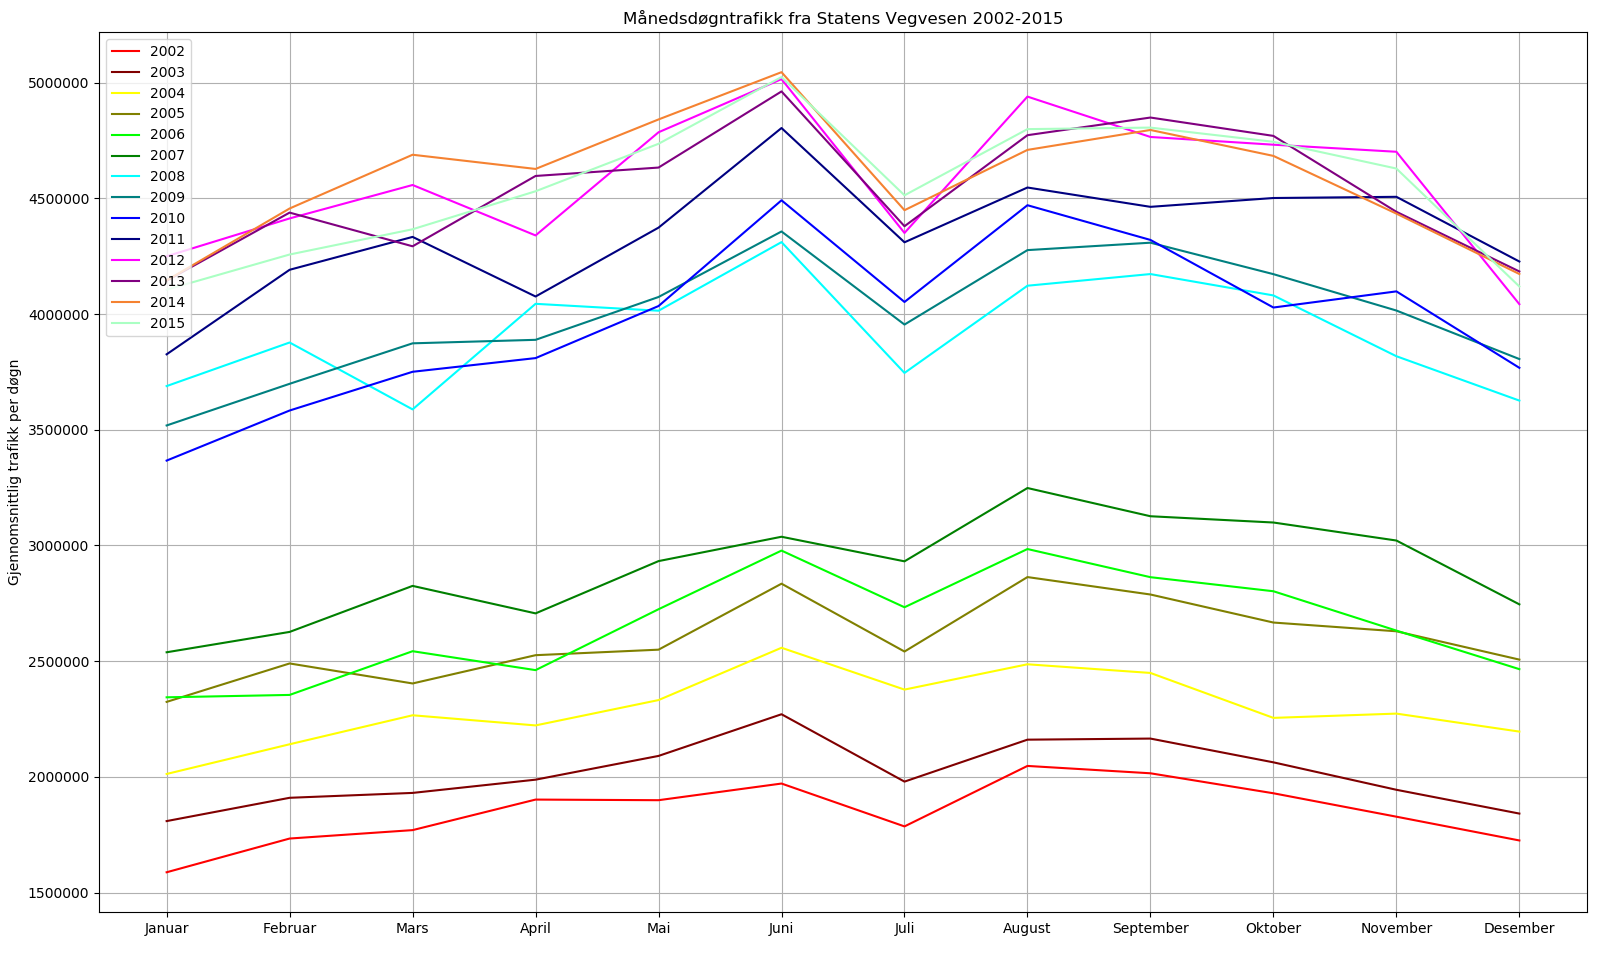
\includegraphics[width=16cm]{xml_02_15_annual_total}
\centering
\caption{Annual traffic 2002-2015}
\label{fig:anualtotal}
\end{figure}

Also derived from this the annual traffic of the two cities Bergen and Oslo, which are towns in interest. Figure \ref{fig:anualbergen} shows the traffic in Bergen, and figure \ref{fig:anualoslo} show the traffic in Oslo.

\begin{figure}[ht]
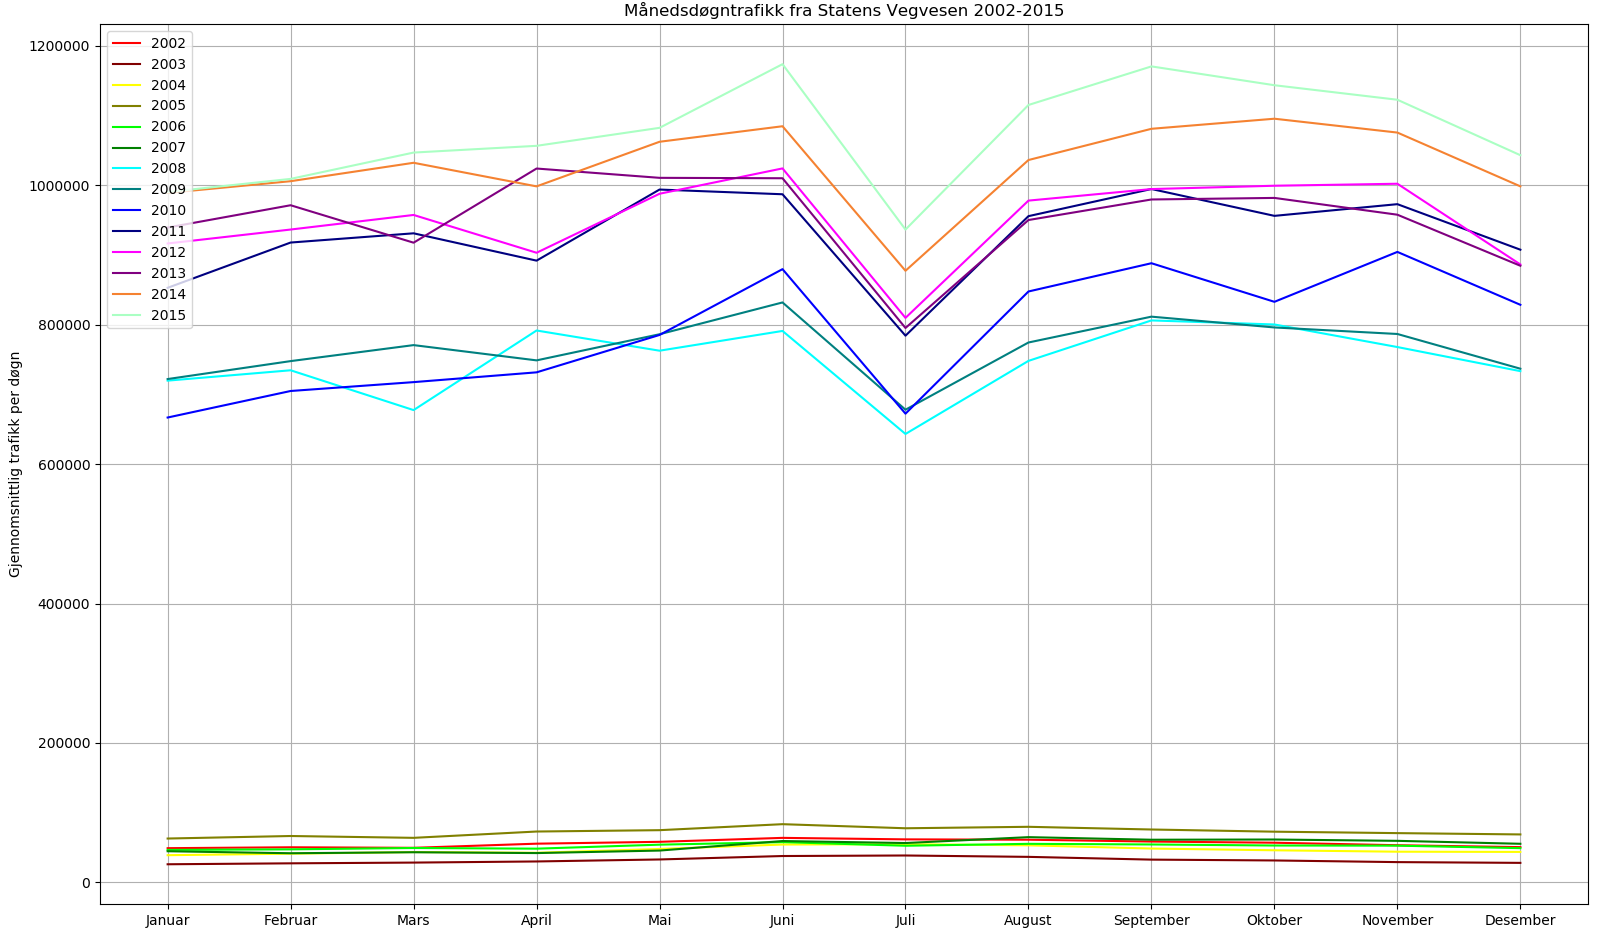
\includegraphics[width=16cm]{xml_02_15_annual_bergen}
\centering
\caption{Bergen traffic 2002-2015}
\label{fig:anualbergen}
\end{figure}

\begin{figure}[ht]
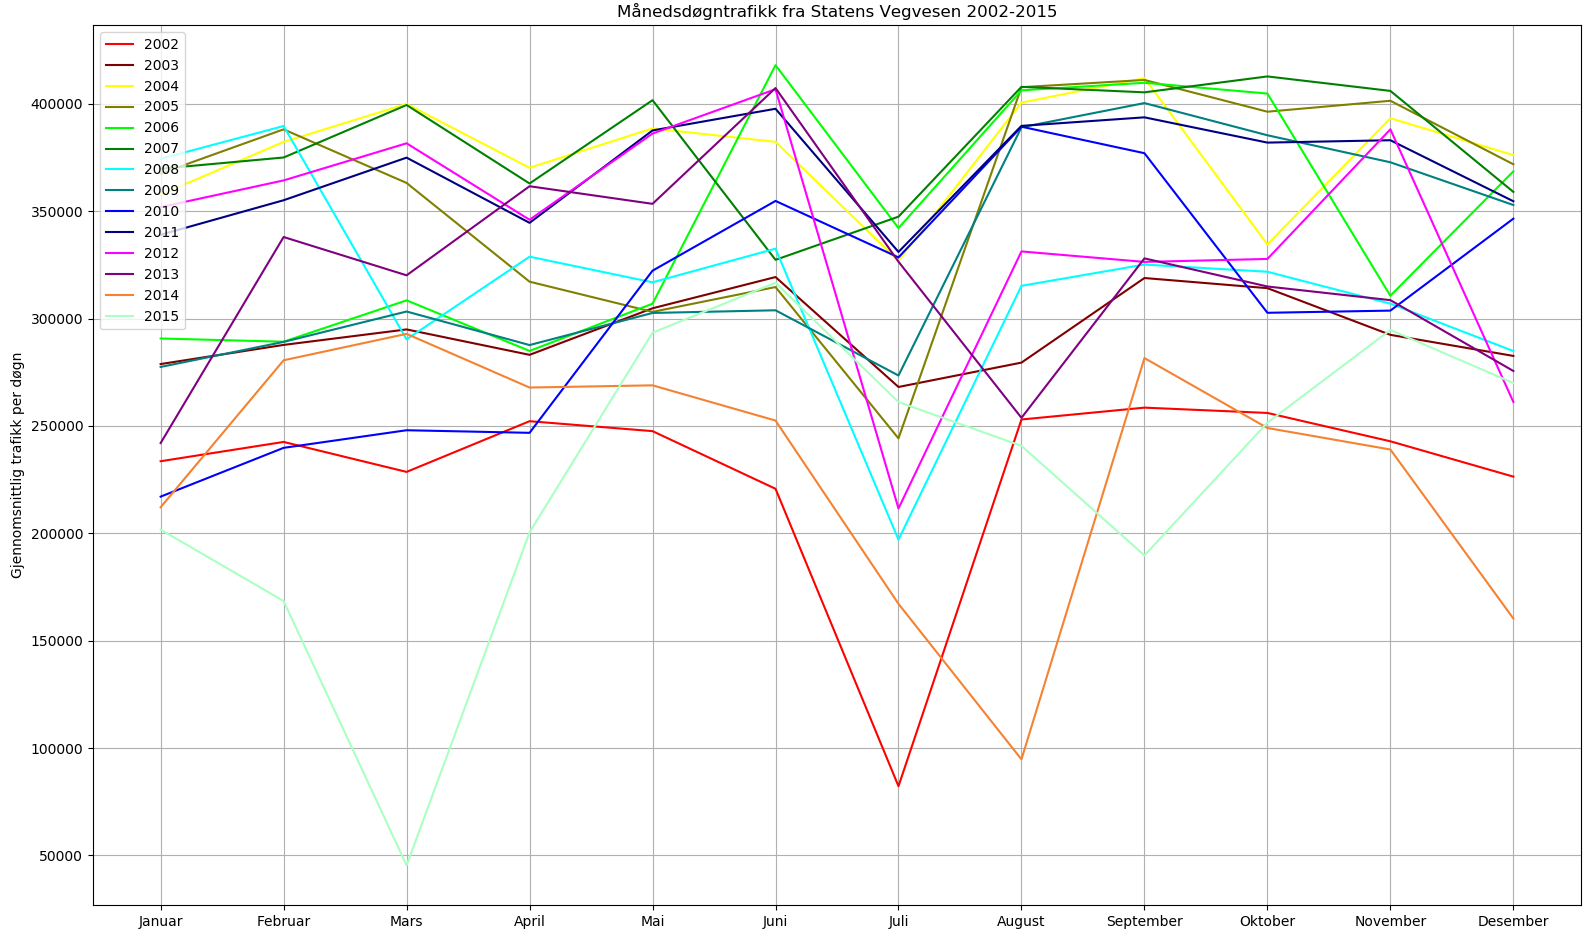
\includegraphics[width=16cm]{xml_02_15_annual_oslo}
\centering
\caption{Oslo traffic 2002-2015}
\label{fig:anualoslo}
\end{figure}
The dataset is an XLM file structure that is downloaded from the NPRA manually. A python program was created that reads through all rows and collects the relevant columns into an array and then draws a graph. For the annual graph every month of every year was collected. For the towns of Bergen and Oslo the correct roads were identified and loaded from a separate text file, then every year of every month of those roads were collected, loaded into an array and the drawn as a graph. The separate text file is to make it easy to edit should these roads change in the future.
The problem of using these datasets is that the data is an average calculation of monthly traffic, this is too coarse for comparison against the influenza data as they are on a weekly basis. Luckily upon further investigation and help from the NPRA better data was accessible upon request, hidden from that available on their website. A set of traffic registration stations was needed to define the temporal bounds of each area of interest. Defined are the towns of Oslo and Bergen, as well as the whole of Norway on a level 1 basis. The level 1 registrations ensures continually registration throughout the year, and is exactly what this project requires.

\newpage\newpage

\section*{4.3 Twitter}
Using the REST search API it was paramount that in order to build a sufficient dataset acquiring and collecting data had to begin as soon as possible. A simple python program was created that takes the input of the API keys and the keywords to be searched upon . The program ensures that no duplicate messages are recorded, and the limit of a hundred tweets was overcome simply by searching for yet another hundred from the last date of the previous hundred, until the date limit was reached.
The output is appended to a file in this format: id, date, location, tweet.

Analysis of the output then need to be divided into categories based on relevant content.

% ------------------------------------------------------------------------------------------------
\chapter*{\vspace{-3cm}5 Results}

\section*{5.1 TODO}

% ------------------------------------------------------------------------------------------------
\chapter*{\vspace{-3cm}6 Discussion}

\section*{6.1 TODO}

% ------------------------------------------------------------------------------------------------
\chapter*{\vspace{-3cm}7 Conclusion}

\section*{7.1 TODO}

% ------------------------------------------------------------------------------------------------
\begin{thebibliography}{1}

\bibitem{fhi.no} fhi.no {\em Influenza statistics from the Norwegian Public Health Institute 		Folkehelseinstituttet}

\bibitem{vegvesen_for_utviklere} https://www.vegvesen.no/om+statens+vegvesen/om+organisasjonen/For+utviklere+API {\em Available data from the NPRA}

\bibitem{norman} TODO: E. H. Norman {\em Japan's emergence as a modern state} 1940: International Secretariat, Institute of Pacific Relations.

\bibitem{fo} TODO: Bob Tadashi Wakabayashi {\em Anti-Foreignism and Western Learning in Early-Modern Japan} 1986: Harvard University Press.

\end{thebibliography}

% ------------------------------------------------------------------------------------------------
\chapter*{\vspace{-3cm}A Appendix}

\section*{A.1 Source Code}

\section*{A.2 TODO}
\end{document}
